\documentclass[conference]{IEEEtran}
\usepackage[T1]{fontenc}
\usepackage{amsmath,amssymb,booktabs,siunitx,graphicx,microtype,xcolor,url}
\usepackage{hyperref}
\usepackage[nameinlink,noabbrev]{cleveref}
\usepackage{tikz,pgfplots}
\usetikzlibrary{arrows.meta,positioning,shapes.geometric}
\pgfplotsset{compat=1.18}
\sisetup{group-separator={,},group-minimum-digits=4}
\newif\ifworkingdraft
\workingdrafttrue

\newcommand{\paperversion}{v0.7}
\newcommand{\papertitle}{Beyond the Wall Horizon: Accuracy-Preserving Search Optimization for High-Branching Quoridor}
\newcommand{\paperauthor}{Author Name}
\newcommand{\paperaffiliation}{Affiliation or independent researcher}
\newcommand{\paperemail}{author@example.com}

\newcommand{\walwuk}{\textsc{walwuk}}
\newcommand{\walper}{\textsc{walper}}
\newcommand{\mainDepth}{\ensuremath{d_{\mathrm{main}}}}
\newcommand{\verifiedDepth}{\ensuremath{d_{\mathrm{verified}}}}
\newcommand{\selDepth}{\ensuremath{d_{\mathrm{sel}}}}
\newcommand{\todoresult}[1]{\ifworkingdraft\textcolor{orange!80!black}{[future result: #1]}\else\PackageError{walwuk-paper}{Unresolved future result: #1}{}\fi}
\newcommand{\preliminary}{\textit{preliminary}}
% Generated by scripts/article-generate.mjs. Do not edit.
\newcommand{\PaperSnapshotId}{phase1-phase2-preliminary-2026-08-12}
\newcommand{\ProductionMask}{0}
\newcommand{\EmscriptenVersion}{6.0.6}
\newcommand{\ParityPositions}{\num{1000000}}
\newcommand{\PhaseOneOldFiveSecondSelectiveDepth}{8}
\newcommand{\PhaseOneNewFiveSecondSelectiveDepth}{10}
\newcommand{\PhaseOneOldFiveSecondVerifiedDepth}{5}
\newcommand{\PhaseOneNewFiveSecondVerifiedDepth}{6}
\newcommand{\PhaseOneOldFifteenSecondSelectiveDepth}{9}
\newcommand{\PhaseOneNewFifteenSecondSelectiveDepth}{11}
\newcommand{\ColdExpectedMoveDepth}{8}
\newcommand{\WarmExpectedMoveDepth}{9}
\newcommand{\ExpectedMoveReusedNodes}{\num{6343}}
\newcommand{\SamePositionReusedNodes}{\num{9950}}
\newcommand{\DynamicRootSingleMs}{\num{7201}}
\newcommand{\DynamicRootEightMs}{\num{1557}}
\newcommand{\DynamicRootSpeedup}{4.63}
\newcommand{\DynamicRootEfficiency}{57.9}
\newcommand{\PilotGames}{\num{2400}}
\newcommand{\PilotHybridWins}{\num{1106}}
\newcommand{\PilotExhaustiveWins}{\num{1277}}
\newcommand{\PilotUnresolved}{\num{17}}
\newcommand{\PilotPlies}{\num{145720}}
\newcommand{\PilotAveragePlies}{60.72}
\newcommand{\PilotScheduledJobs}{8}
\newcommand{\EngineMemoryMiB}{1536}
\newcommand{\ZeroWallStates}{\num{11520}}
\newcommand{\LowWallStateCeiling}{\num{50000}}

% Generated by scripts/article-generate-phase3.mjs. Do not edit.
\newcommand{\PhaseThreeSnapshotId}{phase3-tranche1-preliminary-2026-08-15}
\newcommand{\PhaseThreeProbCutWins}{49}
\newcommand{\PhaseThreeProbCutBaselineWins}{51}
\newcommand{\PhaseThreeProbCutDepth}{7.66}
\newcommand{\PhaseThreeProbCutBaselineDepth}{7.86}
\newcommand{\PhaseThreeMultiCutWins}{50}
\newcommand{\PhaseThreeMultiCutBaselineWins}{50}
\newcommand{\PhaseThreeMultiCutDepth}{7.96}
\newcommand{\PhaseThreeMultiCutBaselineDepth}{8.59}
\newcommand{\PhaseThreeAdaptiveLmrGames}{500}
\newcommand{\PhaseThreeAdaptiveLmrWins}{267}
\newcommand{\PhaseThreeAdaptiveLmrBaselineWins}{233}
\newcommand{\PhaseThreeAdaptiveLmrDepth}{8.66}
\newcommand{\PhaseThreeAdaptiveLmrBaselineDepth}{8.23}
\newcommand{\PhaseThreeParityRandom}{2000}

% Generated by scripts/article-generate-selective-validation.mjs.
\newcommand{\SelectiveValidationSnapshotId}{selective-validation-2026-08-15}
\newcommand{\AggressiveLmrFixedNodeGames}{2000}
\newcommand{\AggressiveLmrFixedNodeScore}{1018--981--1}
\newcommand{\AggressiveLmrRegret}{1300}
\newcommand{\SelectiveBaselineRegret}{1079}
\newcommand{\GuardedLmrFixedNodeGames}{500}
\newcommand{\GuardedLmrFixedNodeScore}{264--236}
\newcommand{\GuardedLmrTimedGames}{100}
\newcommand{\GuardedLmrTimedScore}{62--38}
\newcommand{\GuardedLmrTimedAveragePlies}{53.36}
\newcommand{\GuardedLmrRegret}{1059}


\hypersetup{colorlinks=true,linkcolor=blue!45!black,citecolor=green!35!black,urlcolor=blue!55!black,pdftitle={\papertitle},pdfauthor={\paperauthor}}
\title{\papertitle\\\ifworkingdraft\large Working paper \paperversion---preliminary results\fi}
\author{\IEEEauthorblockN{\paperauthor}\IEEEauthorblockA{\paperaffiliation\\\paperemail}}
\begin{document}
\maketitle
\begin{abstract}
Quoridor has compact rules but an unusually expensive game tree: ordinary positions combine a few pawn actions with up to roughly one hundred structurally available wall actions, and wall legality depends on preserving a route for both players. This working paper describes \walwuk, an accuracy-first engine whose deeper selective search is paired with an exhaustive root verifier. The search core is written in C++, compiled to WebAssembly, and executed in persistent browser workers under explicit processor and memory budgets. Current validated engineering results include zero mismatches in \ParityPositions deterministic rule and path comparisons, an opening selective-depth increase from \PhaseOneOldFiveSecondSelectiveDepth{} to \PhaseOneNewFiveSecondSelectiveDepth{} plies at five seconds, and cross-turn transposition reuse that increased the expected-move search from \ColdExpectedMoveDepth{} to \WarmExpectedMoveDepth{} plies at one second. A preliminary \PilotGames-game campaign currently favors the exhaustive reference and has not crossed its sequential-test boundaries. These results establish a reproducible methodology and implementation baseline; they do not solve full 9$\times$9 Quoridor or establish globally optimal play.
\end{abstract}
\section{Introduction}
Quoridor appears small: two pawns move on a 9$\times$9 board and each player owns ten walls. Its computational structure is not small. A turn can offer only a handful of pawn moves but many wall placements, and a wall is legal only if both players retain a route to their goal. Consequently, generating and evaluating a node may require graph work that has no direct analogue in ordinary chess move generation. Prior full-board programs commonly rely on shallow alpha--beta search or selective Monte Carlo tree search, while recent exact work achieves striking results only on reduced boards~\cite{glendenning2005,slatton2026solver,gorisanson2024}.

\walwuk{} studies how far an accuracy-preserving engine can be pushed under practical browser constraints. The system combines a deep selective lane with an exhaustive root verifier, uses a native C++ core compiled to WebAssembly, and treats every speed or strength optimization as an experiment that must pass deterministic parity and statistical promotion gates. The project targets realistic 10--15 second decisions within a 3 minute plus 1 second competitive clock, rather than maximizing a depth number in isolation.

This working paper makes four presently supported contributions. First, it documents a reproducible hybrid search architecture that distinguishes provisional depth from exhaustively verified depth. Second, it measures exact hot-path changes, transposition reuse, and parallel root search rather than reporting NPS alone. Third, it publishes rejected and inconclusive experiments alongside retained improvements. Fourth, it provides an evolving evidence pipeline in which numerical claims are generated from versioned, checksummed snapshots. Claims of algorithmic novelty and playing superiority are intentionally deferred until broader literature and match evidence support them.

\section{Research Questions and Claims}
The project is organized around questions rather than a single headline NPS target.

\textbf{RQ1: How much exact work can be removed without changing a fixed-depth result?} This includes representation, move generation, pathfinding, symmetry, ordering, and TT reuse. An optimization belongs to this class only when every legal root score and deterministic tie break remain identical to the reference at the tested horizon.

\textbf{RQ2: How much deeper can selective search go without increasing decision regret?} Selective wall generation and pruning can dramatically reduce the effective branching factor, but the omitted continuation may be the only long-term defense. This question is evaluated through exhaustive root regret, fixed-node tests, and paired games rather than displayed depth alone.

\textbf{RQ3: Can an exhaustive verifier make aggressive search practically safer?} The verifier cannot prove lines deeper than its own horizon. It can nevertheless catch shallow tactical contradictions, compare every legal root action at a common depth, and prevent a deep selective result from being presented as uniform coverage.

\textbf{RQ4: How much analysis can be reused across time and moves?} Iterative deepening already reuses ordering within one request. Continuous browser analysis creates a second opportunity: keep workers, TT entries, histories, and a previous principal variation alive; then rebase after the observed move.

\textbf{RQ5: Which metric best predicts playing improvement?} Candidate metrics include NPS, time to depth, effective branching factor, verified depth, selective depth, root regret, PV stability, and paired-game score. The working hypothesis is that no single metric suffices: exactness gates rule out corrupt changes, time-to-depth measures engineering, and equal-resource games measure practical strength.

\textbf{RQ6: What is the performance cost of browser portability?} Native C++ offers a useful reference, but the delivered engine must run as WebAssembly within worker, memory, and hosting restrictions. The paper therefore records artifact identity and compares native and Wasm behavior before attributing a regression to search design.

The present evidence supports only bounded claims. The implementation has passed large sampled parity suites; retained optimizations improve measured depth and reuse on the recorded host; and the hybrid architecture exposes uncertainty more honestly than a single selective number. It is not yet supported that \walwuk{} is the strongest public Quoridor engine, that its preferred move is globally optimal, or that selective search has surpassed the exhaustive reference in statistically controlled play.

\section{Background and Related Work}
At a node with legal actions $A(s)$, negamax searches the value
\begin{equation}
V(s,d)=\max_{a\in A(s)}-V(T(s,a),d-1),
\end{equation}
where $T$ applies an action and $d$ is the remaining nominal depth. Alpha--beta bounds avoid visiting branches that cannot alter the result; iterative deepening supplies ordering information and a usable result when time expires. A transposition table (TT) stores bounds for positions reached by different move orders. Principal-variation search, aspiration windows, history ordering, and selective reductions are established ingredients of high-performance adversarial search~\cite{stockfishSearch,stockfishTT}.

Glendenning developed an iterative-deepening alpha--beta Quoridor program and a domain-specific evaluation~\cite{glendenning2005}. Several public engines provide useful reference points. Dais and Prentzas publish a C alpha--beta engine with iterative deepening, Zobrist hashing, and a TT~\cite{dais2023}. Gorisanson publishes a heuristic MCTS engine that limits expansion to probable wall placements and reports paired match results~\cite{gorisanson2024}. Borowski publishes a generic C++ MCTS implementation demonstrated on Quoridor~\cite{borowski2021}. Slatton's recent MIT-licensed Rust solver precomputes wall configurations and uses proof-oriented search and retrograde analysis to solve reduced boards, but explicitly reports that the method does not scale to full 9$\times$9 play~\cite{slatton2026article,slatton2026solver}. AlphaZero provides a contrasting policy/value-guided search paradigm for difficult evaluation domains~\cite{silver2017}.

% Generated file.
\begin{table*}[t]
\centering
\caption{Public Quoridor search projects considered in the literature review. Evidence is not directly comparable across projects.}
\label{tab:related-work}
\scriptsize
\begin{tabular}{p{0.16\textwidth}p{0.08\textwidth}p{0.16\textwidth}p{0.18\textwidth}p{0.25\textwidth}p{0.07\textwidth}}
\toprule
Project & Board & Language & Search & Published evidence & License \\
\midrule
Glendenning~\cite{glendenning2005} & 9$\times$9 & Java & iterative alpha--beta & thesis methodology; no modern common benchmark & thesis \\
Dais--Prentzas~\cite{dais2023} & 9$\times$9 & C & alpha--beta, TT & competition winner; no NPS/depth protocol & MIT \\
Gorisanson~\cite{gorisanson2024} & 9$\times$9 & JavaScript & heuristic MCTS & rollout counts and paired match tables & MIT \\
Borowski~\cite{borowski2021} & 9$\times$9 & C++ & vanilla MCTS & qualitative competence; no common benchmark & repository license \\
Slatton~\cite{slatton2026solver} & reduced & Rust & proof search, retrograde & reproducible solved small boards; 9$\times$9 out of scope & MIT \\
\walwuk{} & 9$\times$9 & C++/Wasm & hybrid alpha--beta & parity, time-to-depth, root audits, preliminary self-play & MIT \\
\bottomrule
\end{tabular}
\end{table*}


No project in \cref{tab:related-work} publishes a directly comparable full-board benchmark using identical rules, positions, hardware, legal coverage, and node definition. Accordingly, this paper compares \walwuk{} versions against its own exhaustive reference and treats external engines as architectural references until a common protocol is implemented.

\section{Comparative Engine Landscape}
\subsection{Why comparison is unusually difficult}
Engine comparisons are meaningful only when the game rules, root position, resource limit, move coverage, and node definition agree. Public Quoridor projects rarely provide all five. One engine may count an MCTS rollout, another a negamax call, and another a fully evaluated child as one node. A claimed depth of eight may include only walls near a pawn, while a verified depth of six may examine every legal wall at every covered root. Hardware and language further confound raw timing.

For that reason this paper uses three comparison levels. A \emph{feature comparison} asks which mechanisms are documented. A \emph{reproduction comparison} builds an engine and repeats its own published experiment. A \emph{strength comparison} adapts both engines to identical rules and paired controls. At present only the first level is complete for external projects.

\subsection{Classical Quoridor alpha--beta}
Glendenning's thesis is the most important early systematic treatment in the surveyed literature. It describes iterative-deepening negamax and domain-specific evaluation, establishes terminology used by later hobby engines, and emphasizes shortest paths and walls as strategic resources~\cite{glendenning2005}. The public Dais--Prentzas C engine combines alpha--beta, iterative deepening, a TT, Zobrist hashing, and path-based evaluation; its repository reports first place in a local university competition~\cite{dais2023}. The public JavaScript engine by Elmowaled claims depth eight in a few seconds by dynamically restricting wall candidates~\cite{elmowaled2025}. These projects demonstrate viable full-board play, but none publishes an artifact-pinned benchmark corpus comparable to \walwuk's current parity and root-audit records.

Relative to these engines, \walwuk{} documents more extensive reproducibility machinery, separates main and verified depth, uses a C++/Wasm hot path, maintains full packed-position TT verification, and runs large deterministic parity tests. Those are engineering distinctions, not proof of higher Elo. Elmowaled's apparent depth may be reached faster because its wall policy is more selective; without the same candidate set and positions, the number cannot be ranked against \mainDepth{} or \verifiedDepth.

\subsection{Monte Carlo approaches}
Borowski's C++ framework applies vanilla MCTS to Quoridor and discusses the tradeoff between cheap random rollouts and strategically informed simulation~\cite{borowski2021}. Gorisanson reports that pure MCTS played poorly and improved it using probable-wall expansion, shortest-path-biased rollouts, wall-reserve penalties, and a small opening repertoire~\cite{gorisanson2024}. Its strongest published web setting performs 60,000 rollouts and includes paired results against weaker versions and older agents.

MCTS has an attractive property for the wall branching problem: it does not attempt to cover every action uniformly to a nominal depth. It also creates a different failure mode. If a critical wall receives little prior or rollout support, additional simulations may reinforce the wrong region of the tree. \walwuk's verifier provides a type of shallow worst-case protection that heuristic MCTS does not advertise. Conversely, the MCTS engines may capture long-term outcomes through full rollouts that a handcrafted fixed-depth evaluation misses. A fair match, not NPS, is required to decide which advantage matters more.

\subsection{Exact reduced-board solving}
Slatton's solver is the strongest surveyed example of Quoridor-specific exact engineering. On small boards it enumerates wall configurations, precomputes goal-reachability masks, searches for bounded proofs, and falls back to retrograde graph analysis for loops~\cite{slatton2026article,slatton2026solver}. Its published example reports 857,072,712 nodes for a depth-25 5$\times$5 proof. The key insight is not directly portable precomputation: the author estimates roughly $10^{20}$ wall configurations for full 9$\times$9. The portable ideas are bitboard walls, monotonic deferred illegality, symmetry, proof-oriented bounds, and topology-indexed data.

On the small configurations it targets, this solver appears decisively more capable than \walwuk's general game-playing search because it proves complete outcomes. On the full board, it is not a competing player and explicitly disclaims scalability. Thus ``faster'' depends on the task: it is a superior reduced-board solver, while \walwuk{} is designed for full-board, time-limited recommendation.

\subsection{Chess-engine inspiration and limits}
Stockfish supplies mature examples of TT replacement, histories, principal-variation search, pruning, reductions, and statistical promotion~\cite{stockfishSearch,stockfishTT,fishtest}. These mechanisms inspire hypotheses, not copyable constants. Chess has an average branching factor and tactical quietness structure unlike Quoridor's wall phase. Capture-based quiescence has no direct analogue when a consequential wall may be placed almost anywhere. Null-move pruning is especially suspect because passing is illegal and tempo is a primary resource in pawn races.

The relevant Stockfish lesson is procedural: isolate changes, measure them at equal resources, and demand large statistical evidence. \walwuk{} cannot presently match the depth or tuning maturity of Stockfish, and nominal ply is not a cross-game measure of intelligence. Its defensible comparison is that it applies a similar experimental discipline to a different and less developed engine ecosystem.

\subsection{Current comparative position}
Among the surveyed public projects, \walwuk{} appears to have the most extensive combination of full-board WebAssembly deployment, exhaustive root verification, persistent multi-worker analysis, fixed-depth differential testing, root-regret auditing, resource accounting, and published negative experiments. Slatton's project is more advanced as an exact small-board solver; Gorisanson's has clearer external match history; and Stockfish is vastly more mature as an optimized adversarial engine. No evidence yet supports a categorical claim that \walwuk{} plays full-board Quoridor better than every alternative.

\section{Game and Problem Formulation}
Let $S=\{0,\ldots,80\}$ be the pawn squares of a 9$\times$9 board and let $W_h,W_v\subseteq\{0,\ldots,63\}$ encode horizontal and vertical wall placements. A position is
\begin{equation}
s=(p_0,p_1,W_h,W_v,r_0,r_1,t),
\end{equation}
where $p_i$ is a pawn square, $r_i\in[0,10]$ is a wall reserve, and $t$ is the side to move. Periwinkle begins at the bottom and seeks the top row; blossom begins at the top and seeks the bottom row. Wallz uses those color and coordinate conventions, while the underlying rules are two-player Quoridor.

A legal turn is either a legal pawn move or one wall placement. Pawn motion is orthogonal unless adjacency to the opposing pawn permits a straight or diagonal jump under the standard obstruction rules. Walls span two adjacent board edges, may neither overlap nor cross, and must leave at least one path from each pawn to its goal. Reaching a goal row ends the game immediately.

For player $i$, $\delta_i(s)$ denotes the shortest legal pawn-path length under the current wall topology. A ply is one action by one player. A forced outcome is reported only when a complete search or exact solver establishes it; a finite heuristic score is not a proof. An open board has four-neighbor pawn motion but 128 nominal wall identities. Structural conflicts reduce that count, yet ordinary early positions still expose roughly one hundred wall choices~\cite{slatton2026article}. This branching asymmetry makes nominal depth incomparable with chess depth.

\section{Engine Architecture}
The user interfaces are written in React and TypeScript. Analysis runs outside the UI thread: a TypeScript coordinator serializes the position once, dispatches root work to persistent Web Workers, and communicates with a C++ engine compiled through Emscripten to WebAssembly~\cite{emscriptenModularized,wasmCore}. GitHub Pages and the \walper{} extension consume byte-identical engine artifacts in the recorded checkpoint.

\begin{figure}[t]
\centering
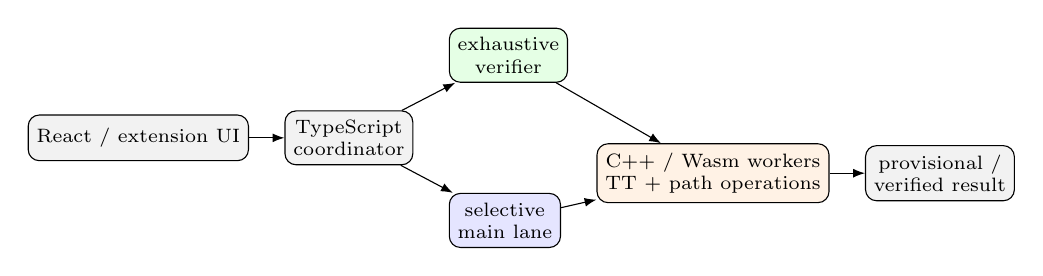
\begin{tikzpicture}[
  node distance=3.5mm and 4.5mm,
  box/.style={draw,rounded corners,align=center,font=\scriptsize,minimum height=5.8mm,inner xsep=3pt},
  arrow/.style={-{Latex[length=1.5mm]},thin}
]
\node[box,fill=gray!10] (ui) {React / extension UI};
\node[box,fill=gray!10,right=of ui] (coord) {TypeScript\\coordinator};
\node[box,fill=blue!10,below right=of coord] (main) {selective\\main lane};
\node[box,fill=green!10,above right=of coord] (verify) {exhaustive\\verifier};
\node[box,fill=orange!10,right=of main,yshift=6mm] (native) {C++ / Wasm workers\\TT + path operations};
\node[box,fill=gray!10,right=of native] (result) {provisional /\\verified result};
\draw[arrow] (ui) -- (coord);
\draw[arrow] (coord) -- (main);
\draw[arrow] (coord) -- (verify);
\draw[arrow] (main) -- (native);
\draw[arrow] (verify) -- (native);
\draw[arrow] (native) -- (result);
\end{tikzpicture}

\caption{Hybrid analysis architecture. The selective lane searches deeper; the verifier searches every legal root action to a shallower common depth.}
\label{fig:architecture}
\end{figure}

The main lane uses selective internal wall generation, reductions, and extensions to provide a deeper provisional principal variation. The verifier assigns every legal root move an exhaustive score at \verifiedDepth. A main result is not described as verified merely because one reduced line reaches \selDepth. Contradictory exhaustive evidence overrides the provisional recommendation.

Workers persist across bounded analysis epochs and retain compatible TT entries, move histories, and principal variations. A board change clears the visible suggestion immediately, while an expected continuation may reuse internal analysis. At most $\lfloor0.75C\rfloor$ heavy workers are scheduled for $C$ reported logical processors, and the count is reduced when the explicit engine-memory budget is tighter. Browser APIs cannot enforce an exact whole-system utilization percentage; the policy limits resources the application can observe and allocate.

\section{Evolution of the Walwuk Engine}
The current architecture was not designed in one pass. It emerged from a sequence of failures in which a locally attractive metric exposed a different weakness.

\subsection{Interactive TypeScript prototype}
The first engine prioritized rule correctness and explainability. TypeScript owned the position, legal pawn movement, wall placement, shortest-path evaluation, and a depth-limited alpha--beta search. That implementation established the application-facing state and move formats, made browser debugging easy, and served as the later native differential oracle. Its main limitation was throughput: allocation-heavy state copying and repeated pathfinding made deeper exhaustive search impractical.

The early interface also treated a completed recommendation as a button-driven event. Continuous analysis later revealed lifecycle requirements that a one-shot calculator did not have: cancellation, stale-result suppression, board-change detection, worker persistence, and the ability to play the latest fully completed move before a longer iteration finishes.

\subsection{C++ and WebAssembly migration}
The search was ported to C++ while UI legality and rendering remained in TypeScript. Compact squares, packed moves, fixed arrays, 64-bit wall masks, precomputed edge masks, and a clustered TT moved the hot path away from JavaScript. The WebAssembly boundary was deliberately coarse: start a search, report periodic progress, and return a result. No JavaScript callback occurs per node.

The TypeScript backend initially remained a fallback and parity reference. This staged migration mattered because a faster engine with subtly different jump or wall rules would have invalidated every later benchmark. Curated positions covered jumps, diagonals, overlaps, crossings, route blocking, low reserves, near wins, and transpositions before native performance became the priority.

\subsection{From exhaustive to plausible search}
Full internal wall generation produced a verified but shallow search. A plausible engine retained all pawn actions and prioritized walls touching a shortest-path witness or lying near either pawn. It added late-move reductions, shallow wall-count pruning, futility conditions, internal iterative reduction, PVS, aspiration windows, and stronger ordering. Initial samples showed two to three more plies at one second, but early matches also demonstrated that greater nominal depth did not guarantee stronger choices.

This led to the hybrid architecture. Every legal root action remained available, the main lane searched plausible continuations more deeply, and an independent exhaustive lane established a shallower common comparison. The interface stopped using one undifferentiated ``depth'' value and exposed main, verified, and seldepth separately.

\subsection{Wall-economy failures}
A conspicuous strategic failure motivated evaluation research: shallow search sometimes spent walls repeatedly to create immediate distance gains, then entered a later phase with only a few walls against a well-stocked opponent. Human advice such as ``do not burn walls early'' described the symptom but was unsafe as a forced rule. Some early walls are tactically decisive.

The preferred formulation became a measurable strategic evaluator: nonlinear value for the last walls, immediate and future wall delay, own-route harm, future anchors, postponability, and the ability to answer the opponent's best wall. The first wall-economy experiment was held rather than promoted because it cost depth and lacked sufficient game evidence. This is representative of the project's policy: theory may suggest features and ordering, but it does not override search.

\subsection{Micro-optimization and misleading NPS}
A concentrated exact pass replaced wall scans with bit operations, precomputed blocked edges and near-pawn masks, reduced temporary move construction, and delayed child path preparation. One-second average NPS improved by 10.2\% for exhaustive and 23.9\% for selective search in the recorded screen. Several apparently reasonable changes failed: larger path and TT caches hurt locality, table-driven pawn neighbors did not beat the hot code, and a structure-of-arrays rewrite added overhead.

These failures reinforced two distinctions. First, a larger cache may produce more hits but lose time through memory traffic. Second, higher NPS may count a cheaper distribution of nodes without completing another useful ply. Consequently, every micro-optimization is judged by fixed-depth parity and time to depth as well as NPS.

\subsection{Parallel extension analysis}
The extension eventually distributed root work over as many as 75\% of reported logical processors. Aggregate NPS rose dramatically, but deterministic modulo partitions created stragglers and duplicated per-worker TT storage. A dynamic exact root queue improved depth-five wall time by 4.63$\times$ on eight workers, yet its 57.9\% efficiency missed the 60\% promotion target. Shared-memory WebAssembly compiled and passed smoke parity, but it did not yet share the TT and therefore offered insufficient benefit to ship.

\subsection{Persistent analysis}
Recreating a worker every turn discarded the TT, histories, Wasm initialization, and the likely continuation of the previous PV. Persistent contexts introduced bounded epochs and start, continue, rebase, cancel, and clear semantics. Reusing the expected continuation gained one completed ply in the recorded one-second opening and exposed reused nodes separately from ordinary TT hits. It also created resource risks: a long-lived pool must be cancelled correctly, bounded by memory, and prevented from treating minor screen-recognition noise as a new game state.

\subsection{Phase Two research discipline}
Phase Two added experiment masks, an immutable promotion manifest, fixed-node matches, campaign checkpointing, model scaffolding, low-wall solvers, native/Wasm parity tooling, and explicit held/rejected states. Importantly, most experiments did not ship. Topology caching, canonical TT symmetry, partial selection, SIMD, and several pruning designs were slower or less stable. The production mask remained zero while evidence accumulated. This history is central to the paper: the research contribution is as much the mechanism for refusing weak optimizations as the successful code paths.

\section{Search Methodology}
\subsection{Position and move operations}
The native engine packs squares and moves into integers and represents each wall orientation with one 64-bit mask. Precomputed masks encode blocked edges, crossings, and same-orientation overlap. Make/unmake updates pawns, reserves, wall masks, side to move, and an incremental Zobrist key. TT entries also retain complete packed-position verification, preventing a hash collision from returning another position's score.

Move generation is staged. Pawn actions and structurally available walls are generated cheaply; expensive path work is delayed until alpha--beta actually searches a candidate. A retained route certificate can prove that a wall leaves a path intact. If the wall intersects that certificate, direct bitboard breadth-first search recomputes reachability and distance. The measured funnel is shown in \cref{fig:path-funnel}.

\begin{figure}[t]
\centering
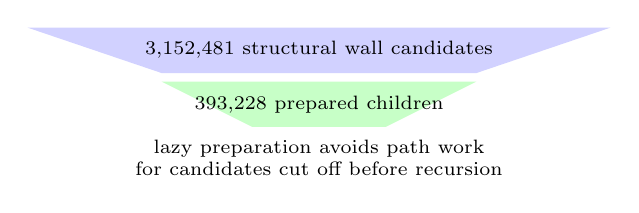
\begin{tikzpicture}[x=1cm,y=0.72cm,font=\scriptsize]
\fill[blue!18] (0,2) -- (7.4,2) -- (5.7,1.2) -- (1.7,1.2) -- cycle;
\fill[green!22] (1.7,1.05) -- (5.7,1.05) -- (4.55,0.25) -- (2.85,0.25) -- cycle;
\node at (3.7,1.62) {3,152,481 structural wall candidates};
\node at (3.7,0.65) {393,228 prepared children};
\node[align=center] at (3.7,-0.3) {lazy preparation avoids path work\\for candidates cut off before recursion};
\end{tikzpicture}

\caption{A diagnostic opening search observed millions of structural wall candidates but prepared only the candidates reached before a cutoff.}
\label{fig:path-funnel}
\end{figure}

\subsection{Tree search and verification}
Production search uses iterative deepening, fail-soft negamax, alpha--beta bounds, principal-variation search, aspiration windows, mate-distance bounds, TT ordering, history, killers, and selective late-move reductions. A reduced search that can improve alpha is re-searched at the required depth and window. Exact left--right root symmetry removes only actions whose scores are mathematically identical under reflection.

At every completed hybrid iteration, the main lane reports \mainDepth{} and the maximum extended line reports \selDepth. The verifier reports \verifiedDepth{} only after all required legal root actions complete. Root positions with no remaining walls can invoke an exact retrograde solver over the fixed-topology pawn-and-turn graph and return a replayable outcome and distance.

\subsection{Production versus experiments}
The production experiment mask is \ProductionMask. Topology caches, alternative histories, strategic evaluation, additional pruning, learned models, canonical TT storage, and all-shortest-route candidates remain individually versioned experiments. Passing parity proves only that an experiment respects the tested rules; it does not promote the experiment. Fixed-node quality, fixed-time performance, tactical regret, and paired strength evidence are separate gates.

\section{Design Alternatives and Rationale}
\subsection{Exhaustive, selective, and hybrid search}
Pure exhaustive alpha--beta offers the cleanest fixed-depth interpretation: every legal continuation is available until the horizon. Its weakness is effective branching factor. Pure selective search spends compute on plausible paths and reaches farther, but its result may depend on an omitted wall. Pure MCTS offers anytime sampling and long rollouts but lacks a common exhaustive horizon. The chosen hybrid is intentionally asymmetric: deep search proposes; exhaustive search challenges.

This does not make the proposal correct. If the decisive refutation lies deeper than \verifiedDepth, both lanes may miss it. The design instead creates an observable confidence boundary. A future confidence model can incorporate root score separation, verifier agreement, PV stability, and regret history without relabeling provisional work as proof.

\subsection{Wall generation policies}
At least five policies have been considered. Full generation retains every structurally and path-legal wall. Witness-path generation retains walls intersecting one current shortest route. All-shortest-route generation uses forward and reverse distances to identify every edge belonging to a shortest path. Tactical generation adds walls near either pawn or existing structures. Learned ordering scores every legal candidate but initially removes none.

One witness is cheap but arbitrary when several equal routes exist. The all-shortest-route experiment reduced a known 151-unit root miss to the accepted 100-unit margin across its audit, but still imposed a 23\% median-NPS cost and changed timed choices. It remains held because improving a shallow audit does not establish game strength. A future staged picker may compute the route union only after cheaper stages fail to cut off.

\subsection{Pathfinding and topology caches}
Pawn moves do not alter the wall topology. In principle, one reverse flood fill per goal can supply distances from all squares, making subsequent pawn nodes cheap. In practice, early eager topology caches admitted many wall layouts that were visited once and displaced useful data. The first versions lost 20--90\% throughput; a delayed two-tier version recovered short-screen speed but lost 25\% average NPS at one second.

The next design must be demand-admitted. Tier one stores compact distance fields only after a second encounter. Tier two adds route unions and strategic features after repeated reuse. A wall move attempts bounded incremental repair and falls back to full flood fill when the affected area is large. Every repaired field is sampled against full recomputation in audit builds. This preserves the underlying insight---topology is reusable---without assuming every encountered topology deserves a cache entry.

\subsection{Legality timing}
Immediate wall validation is simple but pays pathfinding for actions alpha--beta may never search. Route certificates already eliminate some calls safely. Slatton proposes a more aggressive alternative: recurse through most apparently legal walls and discover an illegal branch at a leaf, relying on the monotonic fact that adding walls cannot restore a missing route~\cite{slatton2026article}. This could remove substantial internal move-generation work.

The danger lies in score propagation. An illegal child is not a losing legal move; it is absent from the action set. Null values must propagate until the engine can distinguish an illegal ancestor from a legal node whose child happened to be illegal. TT entries must never cache a bound derived from a malformed action set. The technique will therefore enter only as an exhaustively audited experiment with adversarial near-sealing positions.

\subsection{Evaluation versus proof}
Shortest-path difference is fast and often directionally useful, but it ignores how easily paths can be cut. Wall reserve is useful but phase dependent. Mobility matters near contact but is weak in open positions. The evaluator therefore remains an estimate, even when expressed in integer units.

Exact solvers occupy a separate layer. With no reserves, the wall topology is fixed and the remaining state graph contains only pawn squares and side to move. Retrograde analysis can then prove outcomes and distances. Low-wall solvers expand this region but grow rapidly because each remaining wall branches into many topologies. A proof result may replace heuristic evaluation only when its complete graph or certificate is replayable.

\subsection{Learned components}
A compact learned policy is lower risk than a learned value. Ordering every legal move can improve alpha--beta cutoffs without altering coverage. A learned value changes leaf scores and therefore every pruning decision. The planned sequence is consequently policy first, then a deterministic integer value model blended with exact tactical features. Both require stable labels, symmetry-aware held-out data, artifact versioning, and equal-resource matches. Missing or incompatible weights must fall back to the handcrafted engine.

\subsection{Parallel search models}
Static root splitting is deterministic and easy to verify, but load imbalance grows when a few wall moves are expensive. Dynamic root scheduling reduces stragglers. Lazy SMP with a shared TT may discover useful bounds through diversified searches but requires shared Wasm memory and more difficult race auditing. GitHub Pages cannot conveniently provide the cross-origin isolation required for shared memory, so the common production architecture must retain isolated-worker correctness. The extension may specialize only when it automatically falls back to that baseline.

\section{Experimental Methodology}
Each approved snapshot records an engine commit and artifact hashes, Emscripten version, evaluator, ordering policy, experiment mask, hardware, worker and memory limits, corpus, timing control, and randomization metadata. Generated LaTeX macros and tables derive from those snapshots; the evidence ledger maps prose claims back to their sources.

Five test classes are kept distinct. Fixed-depth parity compares legal actions, path results, static scores, root scores, and deterministic best moves. Fixed-node tests compare search quality at equal work. Fixed-time benchmarks measure NPS and time to completed depth. Paired color-swapped self-play estimates strength while controlling openings and first-player effects. Competitive simulations use a 180-second initial clock, one-second increment, and a 15-second per-move cap.

The correctness corpus contains ten curated fixtures and deterministic random legal positions. The release-scale Phase One gate used \ParityPositions positions split into eight shards. Root audits compare selective recommendations with exhaustive scores and express regret in evaluation units. Optimization promotion uses an SPRT-style sequence with 5\% false-positive and false-negative targets, testing $H_0\leq-2$ Elo against $H_1\geq+5$ Elo. A result marked ``continue'' is inconclusive, not a draw or acceptance.

Timed runs are sensitive to browser warm-up, CPU contention, and thermal state. Therefore, fixed-depth equality is the correctness gate, while repeated same-machine time-to-depth is the primary performance measurement. Aggregate root-worker NPS counts a different search decomposition from a single search, and MCTS rollouts represent different work again; neither is treated as directly comparable node throughput.

\section{Experimental Governance}
\subsection{The promotion ladder}
An idea moves through five states. \emph{Proposed} means it has a rationale but no implementation. \emph{Implemented} means it can be enabled independently. \emph{Held} means it passes available correctness checks but lacks sufficient strength or performance evidence. \emph{Rejected} means a reproducible screen failed. \emph{Promoted} means the production manifest enables it after all applicable gates.

The first gate is deterministic rule parity. The second is fixed-depth exhaustive parity for changes claiming exact equivalence. Selective changes instead face a pruning audit and root-regret comparison. Short fixed-node and 250 ms screens eliminate obviously harmful candidates cheaply. Survivors advance through one-, five-, ten-, and fifteen-second paired matches. Only one experimental mechanism is compared at a time unless the experiment explicitly studies interaction.

This ordering minimizes both false confidence and compute waste. A million-game match cannot redeem a wall-rule bug. Conversely, a parity-perfect rewrite may still be slower and should not enter a strength campaign. The manifest preserves failed experiments so future work does not unknowingly repeat them.

\subsection{Statistical interpretation}
Self-play games are paired by opening and color. The score is separated by engine, color, time control, and game order. Unfinished games are reported as unresolved rather than silently scored as draws because full Quoridor is not assumed draw-free. Sequential testing uses predeclared hypotheses and error targets; stopping because an intermediate score looks attractive would invalidate the test.

Engine games are not independent when they reuse the same opening family, deterministic tie breaks, or cross-game caches. The early Phase Two pilot inherited caches between the outbound and return games, so its first and return scores are published separately and the campaign is not used for promotion. The revised harness clears contexts at game boundaries while preserving reuse between moves inside a game, matching actual deployment.

\subsection{Resource governance}
Every benchmark, campaign, and training process observes the same 75\% scheduling ceiling. On the recorded 16-thread host this permits at most twelve heavy workers, but the 1.5 GiB engine budget limited the pilot to eight concurrent jobs. This is not merely a courtesy feature. Oversubscription can increase aggregate nodes while lowering each engine's completed depth, distort comparisons through thermal throttling, and make Chrome unusable.

Known allocations include Wasm memories, TTs, topology caches, model bytes, and worker buffers. When browser memory APIs are unavailable, the engine uses a conservative fallback rather than inferring unlimited capacity. Allocation failure reduces table size or worker count and retries once. Resource settings become part of the experiment identity.

\subsection{Reproducibility and artifact identity}
Every result intended for the paper is copied from volatile output into an immutable curated snapshot. The snapshot contains engine and documentation commits, Wasm and wrapper hashes, evaluator and policy versions, experiment mask, environment, corpus, and protocol limitations. The paper generator hashes the snapshot again and emits the digest manifest included in the Overleaf archive.

Generated macros prevent prose from silently diverging from tables. Generated plot CSVs prevent a graph from using a different result set than its caption. The evidence ledger maps each important number to a snapshot field and original report. A correction creates a replacement snapshot rather than overwriting the old evidence.

\subsection{Research ethics and user data}
Self-play and synthetic legal positions are the default data sources. Positions observed through the extension do not automatically enter training. A user position may be exported only through an explicit action, and an exported record should exclude account identity, chat, page content, and unrelated screen data. Learned assets must document their provenance and remain within the shipped-data budget.

\section{Preliminary Results}
All results in this section are preliminary unless explicitly described as a completed correctness gate.

\subsection{Correctness and time to depth}
The Phase One release-scale rule, movement, wall-legality, path, and evaluation test completed \ParityPositions deterministic random comparisons with zero mismatches. Ten curated fixtures also matched through exhaustive depth three. These tests establish parity over the sampled state space, not a proof covering every reachable state.

At five seconds from the opening, the selective lane advanced from \PhaseOneOldFiveSecondSelectiveDepth{} to \PhaseOneNewFiveSecondSelectiveDepth{} completed plies, while the exhaustive lane advanced from \PhaseOneOldFiveSecondVerifiedDepth{} to \PhaseOneNewFiveSecondVerifiedDepth{}. At fifteen seconds, selective depth advanced from \PhaseOneOldFifteenSecondSelectiveDepth{} to \PhaseOneNewFifteenSecondSelectiveDepth{}. \Cref{fig:time-depth} plots these opening measurements.

\begin{figure}[t]
\centering
\begin{tikzpicture}
\begin{axis}[
  ybar,bar width=5pt,width=\columnwidth,height=4.2cm,
  ylabel={completed ply},symbolic x coords={5s-selective,5s-verified,15s-selective,15s-verified},
  xtick=data,x tick label style={rotate=28,anchor=east,font=\scriptsize},
  ymin=0,ymax=12,legend style={font=\scriptsize,at={(0.5,1.02)},anchor=south,legend columns=2},
  grid=major
]
\addplot table[x=case,y=before,col sep=comma]{generated/time-to-depth.csv};
\addplot table[x=case,y=after,col sep=comma]{generated/time-to-depth.csv};
\legend{before,Phase One}
\end{axis}
\end{tikzpicture}

\caption{Opening completed depth before and after the Phase One exact hot-path changes. Selective and exhaustive depths measure different coverage.}
\label{fig:time-depth}
\end{figure}

\subsection{Parallelism and reuse}
On the recorded i5-12600KF host, a two-second root-split screen measured the aggregate results in \cref{fig:workers}. These figures do not imply superlinear hardware efficiency because split searches visit different nodes. The dynamic exact root queue reduced a depth-five opening search from \DynamicRootSingleMs{} to \DynamicRootEightMs{} ms with eight workers, a \DynamicRootSpeedup$\times$ speedup and \DynamicRootEfficiency\% efficiency. It remains below the 60\% promotion target.

\begin{figure}[t]
\centering
\begin{tikzpicture}
\begin{axis}[
  width=\columnwidth,height=4cm,xlabel={workers},ylabel={aggregate NPS},
  xtick={1,4,12},scaled y ticks=base 10:-6,y tick scale label code/.code={$\times10^6$},
  ymin=0,grid=major
]
\addplot+[mark=*,thick] table[x=workers,y=nps,col sep=comma]{generated/worker-scaling.csv};
\end{axis}
\end{tikzpicture}

\caption{Aggregate root-worker NPS. Wall-clock completed depth, rather than cross-layout NPS, remains authoritative.}
\label{fig:workers}
\end{figure}

Persistent analysis improved the expected-move opening from \ColdExpectedMoveDepth{} to \WarmExpectedMoveDepth{} completed plies at one second and reused \ExpectedMoveReusedNodes{} nodes. Repeating the same opening reported \SamePositionReusedNodes{} reused nodes. These are cache-reuse measurements, not additional newly searched nodes.

\subsection{Self-play pilot}
The resource-capped pilot completed \PilotGames games and \PilotPlies plies, averaging \PilotAveragePlies{} plies per game. The hybrid won \PilotHybridWins, the exhaustive reference won \PilotExhaustiveWins, and \PilotUnresolved games reached the limit. \Cref{fig:pilot-outcomes} separates wins by engine and color.

\begin{figure}[t]
\centering
\begin{tikzpicture}
\begin{axis}[
  ybar,bar width=10pt,width=\columnwidth,height=4cm,
  ylabel={wins},symbolic x coords={periwinkle,blossom},xtick=data,
  legend style={font=\scriptsize,at={(0.5,1.02)},anchor=south,legend columns=2},
  ymin=0,grid=major
]
\addplot table[x=color,y=hybrid,col sep=comma]{generated/pilot-wins.csv};
\addplot table[x=color,y=exhaustive,col sep=comma]{generated/pilot-wins.csv};
\legend{hybrid,exhaustive}
\end{axis}
\end{tikzpicture}

\caption{Preliminary pilot wins by engine and color over both time controls. Unresolved games are omitted from the bars.}
\label{fig:pilot-outcomes}
\end{figure}

Neither 250 ms nor one-second SPRT crossed a configured boundary. Moreover, this older pilot allowed the color-swapped return game to inherit per-engine caches across a game boundary. The data remain useful as a baseline but cannot promote or reject the hybrid. The updated protocol clears each engine between games while preserving reuse between moves within a game.

\subsection{Negative and held experiments}
The experiment registry in \cref{tab:experiments} records failures rather than selecting only favorable measurements. Eager topology caching, partial selection, several untuned histories, canonical per-node symmetry, and the SIMD build reduced NPS or completed depth. ProbCut, multi-cut, reverse futility, adaptive reductions, strategic evaluation, quiescence, and all-shortest-route candidates remain held because short screens changed preferred moves or lacked strength evidence.

\subsection{Phase Three engineering tranche}
The first Phase Three tranche retained two exact hot-path changes and added same-root iteration continuation. The latter reports the restored completed depth explicitly and is bypassed by strict fixed-depth and fixed-node searches. It passed clear-state and strict-search checks, but its short fixed-time depth gain varied across repeated runs and is therefore not yet reported as a strength or performance improvement.

\Cref{tab:phase-three-pruning} records the first fixed-node selective screens. ProbCut scored \PhaseThreeProbCutWins--\PhaseThreeProbCutBaselineWins and multi-cut scored \PhaseThreeMultiCutWins--\PhaseThreeMultiCutBaselineWins. Both reached lower average depth than their baselines despite modestly higher reported NPS. They were rejected because faster node counting did not translate into deeper or stronger search. Adaptive LMR subsequently led \PhaseThreeAdaptiveLmrWins--\PhaseThreeAdaptiveLmrBaselineWins{} over \PhaseThreeAdaptiveLmrGames{} games and increased average depth from \PhaseThreeAdaptiveLmrBaselineDepth{} to \PhaseThreeAdaptiveLmrDepth{}. At that tranche, this was promising preliminary evidence below the planned game volume; the follow-up below adds fixed-time and accuracy audits.

% Generated file.
\begin{table*}[t]
\centering
\caption{Preliminary Phase Three fixed-node pruning screens. Each move received 50,000 nodes.}
\label{tab:phase-three-pruning}
\scriptsize
\begin{tabular}{lrrrrrrl}
\toprule
Candidate & Games & Cand. & Base & Unres. & Cand. depth & Base depth & Status \\
\midrule
ProbCut & 100 & 49 & 51 & 0 & 7.66 & 7.86 & rejected \\
multi-cut & 100 & 50 & 50 & 0 & 7.96 & 8.59 & rejected \\
reverse futility & 100 & 50 & 50 & 0 & 8.74 & 8.35 & held \\
adaptive LMR & 500 & 267 & 233 & 0 & 8.66 & 8.23 & held \\
\bottomrule
\end{tabular}
\end{table*}

\subsection{Selective-search validation}
A larger follow-up separated playing strength from fixed-depth accuracy.
Aggressive adaptive LMR scored \AggressiveLmrFixedNodeScore{} across
\AggressiveLmrFixedNodeGames{} fixed-node games, but increased summed
depth-five root regret from \SelectiveBaselineRegret{} to
\AggressiveLmrRegret{} over 50 random positions. It therefore remains held
despite its positive match score.

The guarded variant reduced summed regret to \GuardedLmrRegret{}, scored
\GuardedLmrFixedNodeScore{} over \GuardedLmrFixedNodeGames{} fixed-node games,
and scored \GuardedLmrTimedScore{} over \GuardedLmrTimedGames{} games at
250 ms per move. Those timed games averaged \GuardedLmrTimedAveragePlies{}
plies. Neither sequential test crossed a promotion boundary, and representative
timed benchmarks showed no completed-depth gain. A subsequent one-second
screen reversed the short-budget result: guarded LMR scored
\GuardedLmrOneSecondScore{} over \GuardedLmrOneSecondGames{} games, averaging
\GuardedLmrOneSecondAveragePlies{} plies at an aggregate
\GuardedLmrOneSecondNps{} NPS. Guarded LMR was rejected at this non-regression
gate, and the planned five-second screen was not run. The production mask
therefore remains zero.

% Generated file.
\begin{table*}[t]
\centering
\caption{Selective-search validation. Regret is summed over the same 50-position depth-five audit; lower is better. Both SPRTs remained undecided.}
\label{tab:selective-validation}
\scriptsize
\begin{tabular}{lrrr rrl}
\toprule
Variant & Fixed-node games & Fixed-node score & 250 ms games & 250 ms score & Regret & Status \\
\midrule
adaptive LMR & 2000 & 1018--981--1 & 100 & 64--35--1 & 1300 & held \\
guarded LMR & 500 & 264--236--0 & 100 & 62--38--0 & 1059 & held \\
\bottomrule
\end{tabular}
\end{table*}


\subsection{Topology and root scheduling}
The pawn-triggered topology design preserved exact fixture parity but reduced
one-second median NPS from \TopologyVFourBaselineNps{} to
\TopologyVFourCandidateNps{} and average completed depth from
\TopologyVFourBaselineDepth{} to \TopologyVFourCandidateDepth{}. It was
rejected because constructing two reverse fields still cost more than the
saved pawn-path searches.

The sixth dynamic-root prototype uses persistent warm workers, PV-first work,
score-volatility gating, and an exact serial fallback. At depth six, the stable
opening improved by \DynamicRootOpeningSpeedup$\times$ with
\DynamicRootWorkers{} workers, but parallel efficiency was only
\DynamicRootOpeningEfficiency\%. Unstable fixtures used the serial fallback;
an ungated run had previously exposed an equal-score tie divergence and severe
over-search. The guarded scheduler remains held below the 60\% gate.

The shared-memory Wasm artifact compiled and passed parity, but is not enabled.
Independent Emscripten instances cannot safely share their entire linear memory;
a native threaded runtime and explicitly shared caches remain future work.

% Generated file.
\begin{table*}[t]
\centering
\caption{Preliminary depth-six guarded dynamic-root results. Unstable positions use the exact serial fallback.}
\label{tab:phase-five-root}
\scriptsize
\begin{tabular}{llrrrr}
\toprule
Position & Mode & Serial ms & Scheduled ms & Speedup & Move parity \\
\midrule
opening & dynamic & 1803 & 977 & 1.85 & yes \\
channelled routes & serial fallback & 2414 & 2414 & 1.00 & yes \\
transposition rich & serial fallback & 2125 & 2125 & 1.00 & yes \\
\bottomrule
\end{tabular}
\end{table*}

\subsection{Exact TT quality and dynamic-root v7}
Phase 6 corrected clustered TT admission so a matching packed position is
found before an earlier empty slot can create a duplicate. Exact bounds receive
a small replacement preference. Timed search can use a shallow entry's move for
ordering without using its score; strict fixed-depth mode remains isolated from
this cross-search ordering signal. The standard parity screen again reported
zero mismatches.

The one-second ten-position screen preserved the aggregate exhaustive depth and
increased aggregate selective depth from \PhaseSixBaselineSelectiveDepth{} to
\PhaseSixCandidateSelectiveDepth{}. Mean NPS moved slightly downward in that
single run, while the 250 ms run moved slightly upward. The change is retained
for the exact cluster-capacity correction, but these wall-clock results remain
preliminary rather than evidence of a stable speed gain.

Dynamic-root v7 removes the speculative prescreen and first establishes one
exact incumbent. Alternatives are distributed with zero windows, while every
tie or fail-high receives a full-window re-search. The recorded eight-worker
opening improved by \PhaseSevenOpeningSpeedup$\times$ and reduced repeated root
searches from \PhaseSevenPriorRepeatedMoves{} to
\PhaseSevenRepeatedMoves{}. Its \PhaseSevenOpeningEfficiency\% efficiency
still failed the 60\% gate, and a two-worker run was slower than serial search.
Cheap or unstable iterations now use exact serial fallback. The scheduler
therefore remains held and is not connected to the browser or extension.

% Generated file.
\begin{table*}[t]
\centering
\caption{Preliminary depth-six seed-first dynamic-root results on the opening.}
\label{tab:phase-seven-root}
\scriptsize
\begin{tabular}{rrrrrrr}
\toprule
Workers & Serial ms & Scheduled ms & Speedup & Efficiency (\%) & Re-searches & Parity \\
\midrule
2 & 1695 & 1824 & 0.93 & 46.5 & 2 & yes \\
4 & 1663 & 1171 & 1.42 & 35.5 & 3 & yes \\
8 & 1724 & 838 & 2.06 & 25.7 & 4 & yes \\
\bottomrule
\end{tabular}
\end{table*}


\subsection{Shared-memory search and low-wall proofs}
Phase 8 replaced the earlier collection of isolated Wasm instances with an
experimental pthread build whose root searches use one shared linear memory
and one mutex-protected transposition table. Across six depth-four fixtures,
best move, score, and completed depth matched serial exhaustive search. Two
threads produced a median \PhaseEightTwoSpeedup$\times$ speedup at
\PhaseEightTwoEfficiency\% efficiency. Eight threads reached
\PhaseEightEightSpeedup$\times$ but only \PhaseEightEightEfficiency\%
efficiency because duplicated search grew faster than useful parallel work.
The implementation remains held pending extension-context recovery tests and
does not replace the isolated production pool.

Phase 9 added bounded exact AND/OR proof search whose certificates are replayed
independently against legal move generation. In one-total-wall near-goal tests,
it certified a win after a \PhaseNineWinDepth-ply proof while visiting
\PhaseNineWinStates{} states and a loss after a \PhaseNineLossDepth-ply proof
while visiting \PhaseNineLossStates{} states. These proof lengths are replayed
certificate depths, not optimal distances. General one- and two-wall
tablebases remain unfinished, and cycles or budget exhaustion return unknown.

\section{Discussion and Threats to Validity}
NPS is a cost metric, not a strength metric. A selective engine can count cheap, weak nodes or reach a large \selDepth{} through one narrow extension while leaving most alternatives shallow. Conversely, exact wall validation can lower NPS while preventing an illegal or strategically omitted continuation. For this reason \walwuk{} exposes three quantities: \mainDepth{} for the completed selective iteration, \verifiedDepth{} for exhaustive common root coverage, and \selDepth{} for the deepest individual line.

The hybrid still risks overlooking an important internal wall beyond the verifier horizon. Its handcrafted path and reserve evaluation may misjudge delayed wall economy, especially when shallow search rewards early wall pressure. Browser scheduling, WebAssembly implementation, per-worker TT duplication, temperature, and concurrent processes confound timing. The first player and opening corpus may confound self-play. External Quoridor engines use different legality rules, candidate policies, and node definitions, preventing a fair performance ranking without adaptation.

The exhaustive reference's current pilot advantage is informative. It shows that greater selective depth has not yet compensated reliably for omitted internal alternatives and evaluation error. Publishing that result prevents a higher depth display from being mistaken for stronger play and provides a concrete target for pruning audits, evaluator tuning, and fixed-node tests.

No result establishes a globally perfect move, solves the full game, or reaches Stockfish-like semantic depth. Quoridor's wall branching and route computations differ fundamentally from chess captures and quiet positions. The present claim is narrower: the system can improve practical depth while retaining a separately measured floor of exhaustive evidence.

\section{Lessons from Successful and Failed Ideas}
\subsection{Exact optimization should precede aggressive pruning}
Bit masks, precomputed conflicts, make/unmake, lazy child preparation, and compact TT entries improved the cost of work the engine already had to perform. Their fixed-depth behavior could be compared directly. Aggressive pruning offered larger apparent depth gains but also changed moves and sometimes reduced practical strength. The safest development order is therefore to reduce exact cost first, improve ordering second, and omit work only after the audit infrastructure is strong enough to expose misses.

\subsection{Cache admission matters as much as cache lookup}
The engine repeatedly encountered a common optimization trap: a theoretically reusable object was too expensive to build for its actual reuse frequency. Larger TTs, eager topology fields, and broad path caches increased hits or available information while reducing throughput. A useful cache requires a favorable product of reuse probability and saved work, not merely an expensive key. Generation aging, delayed admission, compact entries, and locality can matter more than capacity.

\subsection{A deeper number can conceal less coverage}
The selective engine often reached several more plies than exhaustive search, yet lost the large preliminary pilot. Seldepth could be higher still because one forced line received extensions. These observations are not contradictory. Depth reports the shape of the algorithm, not the probability that its move is correct. A fair assessment also needs legal coverage, root regret, score stability, and match outcome.

\subsection{Human theory is best translated into features and tests}
Advice such as saving walls, blocking routes rather than pawns, keeping one's own lane open, and exploiting jumps is strategically plausible. Encoding it as a forced opening rule can make the engine brittle. Translating it into measurable features creates hypotheses: reserve scarcity, actual path delay, own-path harm, route multiplicity, corridor width, and jump tempo. Search remains free to violate the heuristic when a tactical line justifies the cost.

\subsection{Negative results are cumulative knowledge}
Rejected SIMD, canonical symmetry, topology caching, partial selection, history variants, and pruning designs narrow the future design space. They also reveal the difference between native intuitions and WebAssembly behavior. Recording the exact implementation and screen prevents the project from cycling through the same ideas under new names and makes later revisitation meaningful when surrounding architecture changes.

\subsection{A verifier is a floor, not an oracle}
The exhaustive lane improves honesty and catches shallow contradictions, but it should not be anthropomorphized as certainty. At depth six it knows every legal root continuation for six plies under its evaluation; it does not know the full game. The best suggestion may originate in the deeper lane, the verifier may override it, or both may agree for different horizon-dependent reasons. Confidence must remain tied to what was actually completed.

\subsection{Portability changes the research problem}
A native-only engine could use process threads, unrestricted files, and architecture-specific intrinsics. \walwuk{} must serve both a static GitHub Pages application and a Chrome extension. Worker startup, module loading, shared-memory headers, browser throttling, and memory duplication become algorithmic constraints. The benefit is reproducibility: the same C++ core can be distributed broadly and its artifact hash compared across both interfaces.

\section{Future Research}
The next exact-search studies will test deferred wall legality inspired by Slatton's monotonic-illegality observation, demand-admitted topology caching, dynamic persistent root scheduling, and a shared-memory extension build. All-shortest-route masks will be evaluated at fixed nodes before any candidate omission is widened.

Strength work will tune reductions and pruning one mechanism at a time, improve wall-economy and route-stability features, and train a compact integer policy for ordering only. A value model will be considered after the policy and dataset are stable. Profile-guided native and WebAssembly builds, low-wall retrograde databases, and proof-number search target complementary constant-factor and tactical gains.

External validation will adapt MIT-compatible public engines to a common rules and time-control protocol. Final evidence requires the million-position parity gate on the promoted build, paired 5--15 second campaigns, and competitive 3+1 clock games. \todoresult{report the first statistically completed promotion test and standardized external-engine comparison}

\section{Conclusion}
\walwuk{} is an evolving experiment in accuracy-preserving Quoridor search under browser deployment constraints. Its current implementation combines a selective main search, an exhaustive root verifier, persistent native WebAssembly workers, exact TT identity checks, lazy wall preparation, bounded parallelism, and an exact zero-wall solver. Measurements show substantial time-to-depth and cache-reuse improvements, while the preliminary self-play pilot warns that selective depth alone is not yet stronger than the exhaustive reference. The living-paper workflow ties future claims to versioned evidence and keeps rejected ideas visible. Full-board solution and definitive strength claims remain future work.

\appendices
\section{Terminology and Score Units}
\begin{description}
\item[Main depth.] Deepest completed selective iteration across the main root search.
\item[Verified depth.] Deepest common depth at which every legal root action has exhaustive verifier coverage.
\item[Selective depth.] Synonym for the completed main-search depth in current diagnostics.
\item[Seldepth.] Deepest individual line reached through reductions, re-searches, quiescence, or extensions; not uniform coverage.
\item[Node.] One invocation of the relevant native search routine. Counts are comparable only for the same engine mode and instrumentation.
\item[TT hit.] A position key found in the transposition table. Only usable bounds avoid search; hit count alone does not equal saved nodes.
\item[Evaluation unit.] Handcrafted integer score. One path-equivalent move is provisionally 100 units; this scale is not a calibrated win probability.
\end{description}

\section{Reproducibility}
From the repository root, the following commands regenerate the committed paper assets, validate evidence and references, build locally when a TeX distribution is available, and create an Overleaf ZIP:
\begin{verbatim}
npm run article:generate
npm run article:check
npm run article:build
npm run article:package
\end{verbatim}
The package command places every required source beneath the ZIP root; Overleaf should use \texttt{main.tex}, pdfLaTeX, and BibTeX. Engine validation commands and exact artifact metadata are listed in the evidence ledger and generated snapshot manifest.

The current recorded environment reports an Intel Core i5-12600KF class host with 16 logical processors, Emscripten \EmscriptenVersion, a 12-worker processor ceiling, and a \EngineMemoryMiB\,MiB engine-memory budget. The pilot scheduled \PilotScheduledJobs concurrent jobs because memory constrained the run before the processor ceiling.

\section{Experiment Registry}
% Generated file.
\begin{table*}[t]
\centering
\caption{Versioned search and evaluation experiments. Held means parity passed but strength evidence is insufficient.}
\label{tab:experiments}
\scriptsize
\begin{tabular}{p{0.23\textwidth}p{0.09\textwidth}p{0.58\textwidth}}
\toprule
Experiment & Status & Recorded result \\
\midrule
delayed topology cache v2 & rejected & At 1 s, preserved depth but reduced average NPS by 25\%. \\
continuation/tactical-wall history v2 & rejected & Lost one aggregate ply and changed two of four moves. \\
strategic wall-economy evaluator & held & Lost three aggregate plies; strength evidence required. \\
partial move selection & rejected & Lost two aggregate plies and 32\% average NPS. \\
bounded quiescence & held & Lost three aggregate plies; tactical evidence required. \\
adaptive late-move reductions & held & Changed two of four moves; selective audit required. \\
reverse futility & held & Gained one aggregate ply but changed two of four moves. \\
razoring & rejected & No depth gain and lower average NPS. \\
ProbCut & held & Gained up to three aggregate plies; strength evidence required. \\
history pruning & rejected & No aggregate depth gain. \\
multi-cut & held & Gained two aggregate plies at 1 s; changed two moves. \\
singular extension & rejected & Lost two aggregate plies. \\
forced-defense extension & rejected & No aggregate depth gain. \\
canonical transposition table & rejected & Median NPS fell 32\% and two aggregate plies were lost. \\
all-shortest-route candidates & held & Maximum audited regret fell from 151 to 100; median NPS cost remained 23\%. \\
quantized learned value & untrained & Inference exists; no production-quality dataset or model. \\
\bottomrule
\end{tabular}
\end{table*}


\section{Detailed Pilot Outcomes}
% Generated file.
\begin{table}[h]
\centering
\caption{Preliminary pilot by move-time control.}
\label{tab:pilot-detail}
\scriptsize
\begin{tabular}{rrrrrrl}
\toprule
Limit & Games & Hybrid & Exhaust. & Unres. & Avg. ply & SPRT \\
\midrule
250 ms & 1200 & 536 & 659 & 5 & 59.76 & continue \\
1000 ms & 1200 & 570 & 618 & 12 & 61.67 & continue \\
\bottomrule
\end{tabular}
\end{table}


\section{Proof and Fixture Status}
The final Phase One build passed ten curated fixtures through depth three. A root zero-wall near-win graph completed with \ZeroWallStates states and replayed its proof. The one-total-wall prototype reached a \LowWallStateCeiling-state cap and correctly returned unknown rather than fabricating a result. Future versions will enumerate fixture identifiers and proof-certificate hashes here when those artifacts are frozen for publication.

\section{Algorithm Sketches}
The pseudocode in this appendix documents intent rather than a line-for-line transcription of the optimized C++.

\subsection{Hybrid iterative deepening}
\begin{enumerate}
\item Generate and deterministically order every legal root action.
\item Search the prior-PV or TT root action first in the selective lane.
\item Distribute remaining main-lane root actions within the main work budget.
\item Search every legal root action exhaustively at the next verifier depth.
\item Publish a provisional result whenever a complete main iteration finishes.
\item Publish \verifiedDepth{} only when all verifier root actions at that depth finish.
\item If the verifier contradicts the provisional choice under the configured safety rule, use the verifier choice.
\item Preserve completed iterations, TT entries, histories, and the PV for the next epoch.
\end{enumerate}

\subsection{Fail-soft selective negamax}
Given $(s,d,\alpha,\beta)$:
\begin{enumerate}
\item Stop on a terminal goal and return a distance-adjusted win or loss.
\item Probe the exact-identity TT entry. If its depth and bound permit, return or tighten the window.
\item If $d\leq0$, return the static or bounded tactical evaluation.
\item Construct a staged move picker beginning with TT, PV, immediate-goal, pawn, tactical-wall, and remaining plausible-wall stages.
\item For each selected action, perform structural checks, then make the move and compute path legality only when required.
\item Search the first action with the full window. Search later actions with a null window; re-search a potential improvement.
\item Apply a permitted late-move reduction only outside protected nodes. Re-search any reduced action that raises alpha.
\item Update histories on cutoffs, store a verified TT bound for the exact packed position, undo, and return the fail-soft score.
\end{enumerate}

\subsection{Route-certificate wall validation}
For a structurally non-conflicting wall:
\begin{enumerate}
\item Determine which blocked edges the wall adds.
\item If each player's retained route certificate avoids those edges, the wall preserves both certified routes and is legal.
\item Otherwise, apply the blocked-edge masks and flood-fill from the affected pawn or goal row.
\item Reject the wall if either pawn cannot reach its goal; otherwise cache the new witness when admission policy permits.
\end{enumerate}

\subsection{Persistent rebase}
When a board change is detected:
\begin{enumerate}
\item Cancel the active epoch and invalidate its visible suggestion.
\item Match the observed state against a legal child of the prior root.
\item If engine, evaluator, policy, and representation versions agree, retain compatible TT and histories and reroot the previous PV.
\item Start the new position with the rerooted PV and previous child TT move first.
\item Otherwise clear incompatible caches and start a cold analysis.
\end{enumerate}

\section{Optimization and Experiment History}
This appendix groups ideas by their scientific outcome. A retained change is not necessarily novel; it is a change supported by the project's current parity and performance evidence.

\subsection{Retained exact engineering}
\begin{itemize}
\item C++ search core compiled to modular WebAssembly.
\item Compact 0--80 squares and packed pawn/wall actions.
\item Two 64-bit wall masks with precomputed overlap, crossing, and blocked-edge masks.
\item Incremental Zobrist hashing with full packed-position verification in TT entries.
\item In-place make/unmake and fixed search buffers.
\item Bit-parallel path expansion and cached route witnesses.
\item Structural wall enumeration through masks rather than scanning 128 identities.
\item Lazy child preparation and path computation after move ordering.
\item Iterative deepening, fail-soft alpha--beta, PVS, aspiration windows, and mate-distance bounds.
\item Deeper timed TT bound reuse with strict-horizon parity mode.
\item Exact root reflection reduction in truly symmetric positions.
\item Persistent workers, histories, PV, and TT state across compatible epochs.
\item Root zero-wall retrograde solving with replayable lines.
\end{itemize}

\subsection{Retained selective mechanisms}
\begin{itemize}
\item Every legal pawn action and every legal root action remain available.
\item Internal wall candidates include path-intersecting and near-pawn tactical walls.
\item Later, low-priority walls receive depth-sensitive reductions or shallow omission under guarded conditions.
\item A reduced action that can improve alpha is searched again at the required depth.
\item The exhaustive verifier is kept separate from selective coverage.
\end{itemize}

\subsection{Held ideas}
Held work includes strategic wall-economy evaluation, bounded Wallz quiescence, adaptive reductions, reverse futility, ProbCut, multi-cut, all-shortest-route candidates, dynamic root scheduling, and shared-memory workers. These ideas either gained depth, reduced a known regret, or passed parity, but changed decisions or missed a performance/strength threshold. They remain available for controlled experiments rather than production defaults.

\subsection{Rejected ideas}
The current architecture rejected eager topology caching, an untuned continuation/tactical history, internal zero-wall solving at every frontier, partial selection, correction history, razoring, history pruning, first-generation singular and forced-defense extensions, per-node canonical TT reflection, and the tested Wasm SIMD build. Earlier exact work also rejected table-driven pawn neighbors, structure-of-arrays reconstruction, a four-times-larger path cache, and a doubled TT. Rejection applies to the measured design, not necessarily the general idea; a materially different implementation requires a new experiment identity.

\subsection{Ideas not yet implemented}
Open proposals include monotonic deferred legality on full-board search, demand-admitted incremental topology repair, shared TT Lazy SMP, proof-number search near goals, one- and two-wall databases, a learned integer ordering policy, an NNUE-style value, PGO, tiled 3$\times$3 pathfinding, illegality-frontier indexing, compact opening transpositions, and standardized external-engine adapters.

\section{Planned External-Engine Comparison Protocol}
The statement that one engine ``beats'' another will be reserved for a completed common-protocol match.

\subsection{Rules adapter}
Each engine must use the same 9$\times$9 two-player rules, jump and diagonal-jump conditions, wall coordinates, crossing and overlap rules, ten-wall reserves, immediate goal termination, and no post-win actions. Before matches, a protocol adapter must pass the common legal-action fixtures and at least 100,000 random position comparisons. Engines with irreconcilable rule differences are reported qualitatively only.

\subsection{Resource controls}
Matches use one process or equivalent worker allocation per engine, identical logical-core ceilings, and explicit memory limits. Required controls are fixed node budgets where node semantics permit, 250 ms, one second, five seconds, ten seconds, fifteen seconds, and a 180+1 clock with a fifteen-second move cap. Warm-up occurs before measurement, and caches are cleared at game boundaries but retained between moves within a game.

\subsection{Opening and color control}
Openings are deterministic, legal, and sampled from empty-board, pawn-first, balanced-wall, tactical, low-reserve, and human-derived categories. Every opening is played twice with colors exchanged. Reports separate periwinkle and blossom wins, first and return games, unresolved games, plies, remaining walls, backward pawn actions, and wall usage by phase.

\subsection{Search telemetry}
Where available, the adapter records wall-clock time, nodes or rollouts, completed depth, selective depth, principal variation, memory, and worker count. Metrics whose definitions differ remain in separate columns. The primary result is paired game score with confidence or sequential-test status. Secondary results are root regret against a longer common verifier and move agreement by position class.

\subsection{Interpretation}
A statistically positive match would support ``stronger under this protocol,'' not ``universally stronger.'' A faster time to depth supports an engineering claim only when legal coverage and evaluation are comparable. A proof solver outranks a heuristic engine on positions it proves, regardless of its NPS. All source licenses and modifications will be reported.

\section{Living-Paper Maintenance Protocol}
The manuscript is intended to grow with the engine and eventually reach approximately 30--40 pages including appendices. Length is a consequence of accumulated evidence, not a reason to duplicate prose.

Each major optimization phase adds four artifacts: an immutable snapshot, regenerated tables and plots, a short narrative explaining the hypothesis and outcome, and an updated limitations paragraph. A rejected experiment still receives a registry entry and enough implementation detail to reproduce the rejection. A promoted experiment updates the production manifest, architecture description, result tables, abstract, and conclusion.

The paper version follows a working sequence. Minor versions add experiments or prose without changing the central claim. A major preprint version freezes engine artifacts and completes the release gates. Author metadata remains editable in \texttt{metadata.tex}; changing draft mode off converts unresolved future-result markers into build errors.

The expected final page allocation is approximately four pages for motivation, background, and comparisons; three for rules and formalization; six for architecture and search; four for engine evolution and design alternatives; five for experimental methods and governance; six to eight for final results; four for discussion and future research; and the remaining pages for appendices, reproducibility, algorithms, experiment history, and proof material. This allocation will be revised after the first locally rendered PDF exposes actual IEEE column flow.

\bibliographystyle{IEEEtran}
\bibliography{references}
\end{document}
